\section{Durchführung}
\label{sec:Durchführung}

Der Versuch wird nach \autoref{fig:aufbau} aufgebaut und es wird ein grüner Laser mit einer Wellenlänge von $\SI{532}{\nano\meter}$ verwendet. 
Es wird in Abhängigkeit von sieben verschiedenen Einfallswinkeln der Reflexionswinkel aufgenommen, um das Reflexionsgesetz zu untersuchen.
Bei allen Experimenten ist das optisch dünnere Medium Luft mit der Lichtgeschwindigkeit $c\approx \SI{2,9979}{e8\meter\per\second\squared}$ und dem Brechungsindex $n\approx 1$.
Die \autoref{fig:optischElemente} zwigt die in dem Versuch verwendeten optischen Elemente.

\begin{figure}[H]
    \centering
    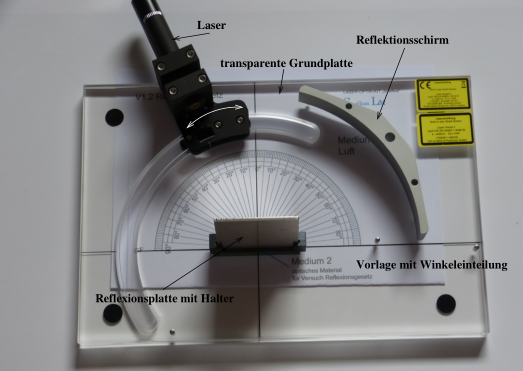
\includegraphics[width=0.7\textwidth]{data/aufbau1.png}
    \caption{Abbildung des Versuchaufbaus Reflexion \cite{Anleitung400}.}
    \label{fig:aufbau}
\end{figure}

\begin{figure}[H]
    \centering
    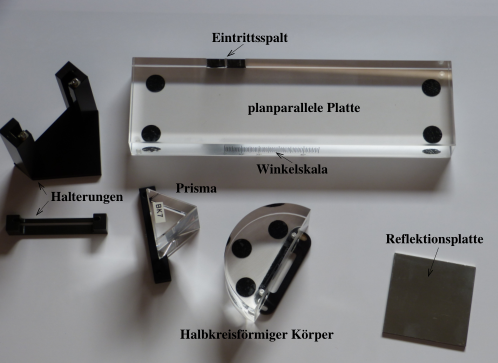
\includegraphics[width=0.7\textwidth]{data/optischeElemente.png}
    \caption{Abbildung der optischen Elemente \cite{Anleitung400}.}
    \label{fig:optischElemente}
\end{figure}

\noindent
In einem zweiten Teil soll das Brechungsgesetz untersucht werden, wofür die planparallele Platte mit dem Eintrittsspalt und der Winkelskala verwendet wird und sie den Winkelskala
vorne anzeigt. Es wird nun für sieben verschiedene Einfallswinkel der Brechungswinkel bei rotem Licht mit einer Wellenlänge von $\SI{635}{\nano\metre}$ gemessen. \newline
Es soll nun das optische Prisma aus \autoref{fig:optischElemente} untersucht werden. Dazu wird es auf der Messapparatur angebracht und es wird für fünf verschiedene Einfallswinkel der
jeweilige Austrittswinkel gemessen werden. Dazu sollen Einfallswinkel aus einem Winkelbereich von $\SIrange{10}{60}{\degree}$ verwendet werden. Die essungen werden sowohl für den roten,
als auch für den grünen Laser durchgeführt.\newline
Als letztes soll die Beugung an drei verschiedenen Gittern unterscuht werden, wozu das Prisma gegen das zu untersuchende Gitter ausgetauscht wird. Es ist darauf zu achten, dass der Laser bei einem Winkel von $0°$ auf das
Gitter trifft und der Transmissionsschirm im Kreis um die Winkelskala der Vorlage angeordnet ist. Es sollen nun die Beugungsmaxima für rotes und grünes Laserlicht gemessen werden.